\documentclass[10pt]{article}

\usepackage{commands}
\pgfplotsset{compat=1.18}
\hypersetup{colorlinks = true}

\begin{document}

\section{PHY509 – Problem Set 2}

\subsection*{Problem 1}
\begin{quote}
	Let $X, Y$ be independent random variables. The Conditional Expectation Formula is:
	$$ \mathbb{E}(X)=\mathbb{E}(\mathbb{E}(X|Y)) $$
	To be clearer, we can explicitly denote which variable the expectation is with respect to as follows:
	$$ \mathbb{E}_{X}(X)=\mathbb{E}_{Y}(\mathbb{E}_{X}(X|Y)) $$
	\begin{enumerate}
		\item[(a)] Prove this for the case of discrete X, Y.
		\item[(b)] Suppose you are playing a computer game in which you are stuck in a room with 3 exits that are indistinguishable, which means you have equal probability of choosing exit 1, 2 or 3. If you leave via exit 1, you get free after traversing 3 other rooms. If you leave via exit 2, you end up back at this same starting room after traversing 5 rooms. If you leave via exit 3, you end up back at this same starting room after traversing 7 rooms. Sadly, if you get back to the room, you are so disoriented that you can't tell which exit you chose last time, so you randomly pick again. How many rooms do you visit on average before getting free? (Bonus: how annoying is the game designer?)
	\end{enumerate}
\end{quote}

\divider

\begin{enumerate}[label=(\alph*)]
	\item Let's prove this by showing that the right hand side equals the left hand side and also using the definition of expectation value for discrete random variables.
	      \begin{equation*}
		      E(X) = \sum_{i} x_i P(X=x_i)
	      \end{equation*}

	      We want to expand out the inner expectation value first:
	      \begin{equation*}
		      E_{X}(X|Y=y) = \sum_{i} x_i P(X=x_i|Y=y)
	      \end{equation*}


	      Plugging that back into the outer expectation value and also using the definition of expectation value for discrete random variables again:

	      \begin{equation*}
		      E_{Y}(E_{X}(X|Y)) = \sum_{j} \left( \sum_{i} x_i P(X=x_i|Y=y_j) \right) P(Y=y_j)
	      \end{equation*}

	      From conditional probability we have:

	      \[
		      P(E|F) = \frac{P(E \cap F)}{P(F)} \quad \text{for } P(F) > 0
	      \]

	      \[ P(E|F) P(F) = P(E \cap F) = P(E,F) \]

	      Such that we can write our expectation expression in terms of the joint probability:
	      \[ E_{Y}(E_{X}(X|Y)) = \sum_{j} \sum_{i} x_i P(X=x_i, Y=y_j) \]

	      For independent events (like for the case of X and Y here) we have $P(A \cap B) = P(A)P(B)$ so that:

	      \[ E_{Y}(E_{X}(X|Y)) = \sum_{j} \sum_{i} x_i P(X=x_i) P(Y=y_j) \]

	      We can move over the terms to their respective sums:

	      \[ E_{Y}(E_{X}(X|Y)) = \sum_{i} x_i P(X=x_i) \sum_{j} P(Y=y_j) \]

	      From the laws of probability we have the law of total probability which states that the sum of the probabilities of all possible outcomes of a random variable is equal to 1, which means that $\sum_{j} P(Y=y_j) = 1$.

	      \[ \boxed{E_{Y}(E_{X}(X|Y)) = \sum_{i} x_i P(X=x_i) \cdot 1 = \sum_{i} x_i P(X=x_i) = E(X) }\]

	\item Let's let X be the number of rooms visited before getting free and Y be the exit chosen.

	      Just to get the problem setup let's remind ourselves of the exit options from the starting room:

	      \begin{itemize}
		      \item Exit 1: 3 rooms to freedom
		      \item Exit 2: 5 rooms then back to start
		      \item Exit 3: 7 rooms then back to start
	      \end{itemize}

	      The question is asking for the expected number of rooms visited before getting free, which is $E(X)$. So using the problem 1 setup let's use the conditional expectation formula we just proved and see if it can help us break down the problem:

	      \[ E_{X}(X) = E_{Y}(E_{X}(X|Y)) \]

	      Putting this into the definition of expectation value for discrete random variables:

	      \[ E_{X}(X) = \sum_{j} \sum_{i} x_i P(X=x_i|Y=y_j) P(Y=y_j) \]

	      Since there are 3 exits that are indistinguishable we have $P(Y=y_j) = \frac{1}{3}$ for $j=1,2,3$.

	      \[ E_{X}(X) = \frac{1}{3} \sum_{j} \sum_{i} x_i P(X=x_i|Y=y_j) \]

	      Putting the expectation value notation back in here will make it easier.
	      \[ E_{X}(X) = \frac{1}{3} \sum_{j} E_{X}(X|Y=y_j) \]

	      Now we need to figure out $E_{X}(X|Y=y_j)$ for each exit choice $j$.

	      \begin{itemize}
		      \item For exit 1 we have $E_{X}(X|Y=1) = 3$ since we just go through 3 rooms and get free.
		      \item For exit 2 we have $E_{X}(X|Y=2) = 5 + E_{X}(X)$ since we go through 5 rooms and then end up back at the starting room.
		      \item For exit 3 we have $E_{X}(X|Y=3) = 7 + E_{X}(X)$ using the same reasoning as exit 2.
	      \end{itemize}

	      Plugging this all in to our expression we have:

	      \[ E_{X}(X) = \frac{1}{3} \left( 3 + (5 + E_{X}(X)) + (7 + E_{X}(X)) \right) \]

	      \[ E_{X}(X) = \frac{1}{3} \left( 15 + 2E_{X}(X) \right) \]

	      Rearranging we have:

	      \[ 3E_{X}(X) - 2E_{X}(X) = 15 \]

	      \[ \boxed{ E_{X}(X) = 15 } \]

	      So on average we visit 15 rooms before getting free. The game designer is very annoying!
\end{enumerate}

\subsection*{Problem 2}
\begin{quote}
	Calculate the characteristic function of a Gaussian of variance $\sigma^{2}$ and show it is a Gaussian of variance $\frac{1}{\sigma^{2}}$.
\end{quote}

\divider

The characteristic function is defined as:

\[ \phi(t) = \mathbb{E}(e^{itX}) = \int_{-\infty}^{\infty} e^{itx} p(x) dx \]

We can the plug in the Gaussian pdf with mean $\mu$ and variance $\sigma^2$:

\[ p_{\text{Gaussian}}(x) = \frac{1}{\sqrt{2\pi\sigma^2}} e^{-\frac{(x-\mu)^2}{2\sigma^2}} \]

\[ \phi(t) = \int_{-\infty}^{\infty} e^{itx} \frac{1}{\sqrt{2\pi\sigma^2}} e^{-\frac{(x-\mu)^2}{2\sigma^2}} dx \]

I used a LLM to generate MATLAB code to solve the integral symbolically:

\begin{verbatim}

	% Define symbolic variables
syms x t mu sigma real
assume(sigma > 0)

% Define the integrand
integrand = exp(1i*t*x) * (1/sqrt(2*pi*sigma^2)) * exp(-(x-mu)^2/(2*sigma^2));

% Compute the integral from -inf to +inf
result = int(integrand, x, -inf, inf);

% Simplify the result
result_simplified = simplify(result);

% Display the result
disp('Result:')
disp(result_simplified)

% Convert to LaTeX
latex_result = latex(result_simplified);
disp(' ')
disp('LaTeX code:')
disp(latex_result)

% Pretty print in MATLAB
disp(' ')
disp('Pretty form:')
pretty(result_simplified)
\end{verbatim}

This gives the result:


\[ \boxed{\phi(t) ={\mathrm{e}}^{-\frac{\sigma ^2\,t^2}{2}+\mu \,t\,1{}\mathrm{i}}}\]

This is a Gaussian (in t) with variance $\frac{1}{\sigma^2}$ and mean $\mu$ and an additional complex exponential factor. And if the mean is $\mu = 0$ then the imaginary term dissapears and we get just $\phi(t) = {\mathrm{e}}^{-\frac{\sigma ^2\,t^2}{2}}$

\subsection*{Problem 3}
\begin{quote}
	\begin{enumerate}
		\item[(a)] Show that, if the characteristic functions for two independent random variables X, Y are $\phi_{X}(t)$ and $\phi_{Y}(t)$, then the characteristic function for the random variable made from the sum, $Z=X+Y$, is just the product $\phi_{Z}(t)=\phi_{X}(t)\phi_{Y}(t)$.
		\item[(b)] If $X_{1}$, $X_{2}$ are two independent Gaussian random variables with means $\mu_{1}$, $\mu_{2}$ and variances $\sigma_{1}^{2}$, $\sigma_{2}^{2}$, prove that the random variable $Y=a_{1}X_{1}+a_{2}X_{2}$ ($a_{i}\in\mathbb{R}$) is Gaussian with mean $\mu=a_{1}\mu_{1}+a_{2}\mu_{2}$ and variance $\sigma^{2}=a_{1}^{2}\sigma_{1}^{2}+a_{2}^{2}\sigma_{2}^{2}$.
	\end{enumerate}
\end{quote}

\divider

\begin{enumerate}[label=(\alph*)]
	\item We start with the definition of the characteristic function for Z:

	      \[ \phi_{Z}(t) = \mathbb{E}(e^{itZ}) = \mathbb{E}(e^{it(X+Y)}) \]

	      This can be rewritten as:

	      \[ \phi_{Z}(t) = \mathbb{E}(e^{itX} e^{itY}) \]

	      Since X and Y are independent random variables, so we can also say that $e^{itX}$ and $e^{itY}$ are independent. Thus, from the independence condition, we can factor the expectation:

	      \[ \phi_{Z}(t) = \mathbb{E}(e^{itX}) \mathbb{E}(e^{itY}) = \phi_{X}(t) \phi_{Y}(t) \]

	      Thus, we have shown that:

	      \[ \boxed{\phi_{Z}(t) = \phi_{X}(t) \phi_{Y}(t)} \]

	\item From Problem 2, we know that the characteristic function of a Gaussian random variable $X_i$ with mean $\mu_i$ and variance $\sigma_i^2$ is given by:

	      \[ \phi_{X_i}(t) = e^{-\frac{\sigma_i^2 t^2}{2} + i\mu_i t} \]

	      We can then consider the random variable $Y = a_1 X_1 + a_2 X_2$. The characteristic function of Y is:

	      \[ \phi_Y(t) = \mathbb{E}(e^{itY}) = \mathbb{E}(e^{it(a_1 X_1 + a_2 X_2)}) = \mathbb{E}(e^{i a_1 t X_1} e^{i a_2 t X_2}) \]

	      Using the independence of $X_1$ and $X_2$, we can factor this expectation:

	      \[ \phi_Y(t) = \mathbb{E}(e^{i a_1 t X_1}) \mathbb{E}(e^{i a_2 t X_2}) = \phi_{X_1}(a_1 t) \phi_{X_2}(a_2 t) \]

	      Substituting the characteristic functions for $X_1$ and $X_2$

	      \[ \phi_Y(t) = e^{-\frac{\sigma_1^2 (a_1 t)^2}{2} + i\mu_1 (a_1 t)} e^{-\frac{\sigma_2^2 (a_2 t)^2}{2} + i\mu_2 (a_2 t)} \]

	      Combining the exponents, we get:

	      \[ \boxed{\phi_Y(t) = e^{-\frac{(a_1^2 \sigma_1^2 + a_2^2 \sigma_2^2) t^2}{2} + i(a_1 \mu_1 + a_2 \mu_2) t}} \]

	      This is the characteristic function of a Gaussian random variable with mean $\mu = a_1 \mu_1 + a_2 \mu_2$ and variance $\sigma^2 = a_1^2 \sigma_1^2 + a_2^2 \sigma_2^2$, which also means that the random variable $Y= a_1 X_1 + a_2 X_2$  ($a_{i}\in\mathbb{R}$) is

	      \[ \boxed{Y \sim \mathcal{N}(a_1 \mu_1 + a_2 \mu_2, a_1^2 \sigma_1^2 + a_2^2 \sigma_2^2)} \]

\end{enumerate}


\subsection*{Problem 4}
\begin{quote}
	\begin{enumerate}
		\item[(a)] Show that the characteristic function for a Poisson is
		      $$ \phi(t)=\sum_{r=0}^{\infty}e^{itr}P(r;\mu)=\exp(\mu(e^{it}-1)) $$
		      and check that you get the right mean and variance from the characteristic function.
		\item[(b)] Use this to show that the sum of two Poisson random variables with means $\mu_{X}$, $\mu_{Y}$ is a Poisson with mean $\mu_{X}+\mu_{Y}$.
		\item[(c)] Prove this the hard way, by computing this directly from the formulas for the Poissons. Note how much easier it was to prove using the characteristic functions!
	\end{enumerate}
\end{quote}

\divider

\begin{enumerate}[label=(\alph*)]
	\item Starting with the definition of the characteristic function

	      \[\phi_X(t) = E[e^{itX}] = \begin{cases} \int_{-\infty}^{\infty} e^{itx} f_X(x) \,dx & \text{for continuous } X \\ \sum_{k} e^{itx_k} p_X(x_k) & \text{for discrete } X \end{cases} \]

	      Recall the Poisson distribution definitions:

	      \[ P(X = k) = \frac{\lambda^k e^{-\lambda}}{k!} \]
	      \[ E[X] = \lambda, \quad \text{Var}(X) = \lambda \]

	      The discrete Poisson random variable for this question has the PMF of:

	      \[ P(r;\mu) = \frac{\mu^r e^{-\mu}}{r!} \]

	      So our characteristic function becomes

	      \[ \phi(t) = \sum_{r=0}^{\infty} e^{itr} P(r;\mu) \]

	      We have:

	      \[ \phi(t) = \sum_{r=0}^{\infty} e^{itr} \frac{\mu^r e^{-\mu}}{r!} = e^{-\mu} \sum_{r=0}^{\infty} \frac{(\mu e^{it})^r}{r!} \]

	      recall the Taylor series expansion for $e^x$:

	      \[ e^x = \sum_{r=0}^{\infty} \frac{x^r}{r!} \]

	      We can rewrite the characteristic function as:

	      \[ \boxed{\phi(t) = e^{-\mu} e^{\mu e^{it}} = e^{\mu (e^{it} - 1)} }\]

	      Recall that the one of the properties of characteristic functions is that the nth moment of the distribution can be found by taking the nth derivative of the characteristic function and evaluating it at t=0:

	      \[ E[X^n] = \frac{1}{i^n} \phi_X^{(n)}(0) \]

	      To find the mean and variance, we then just compute the first and second derivatives of $\phi(t)$ at $t=0$:

	      I used a LLM to generate MATLAB code to compute the derivatives symbolically:

	      \begin{verbatim}
			% Define symbolic variables
			syms t mu real
			assume(mu > 0)

			% Define the characteristic function for Poisson
			phi = exp(mu*(exp(1i*t) - 1));

			% Compute first derivative
			phi_1 = diff(phi, t);

			% Evaluate first derivative at t=0
			phi_1_at_0 = subs(phi_1, t, 0);

			% Compute second derivative
			phi_2 = diff(phi, t, 2);
		\end{verbatim}

	      That MATLAB code gives me the following equations:


	      \[ \phi(t) = {\mathrm{e}}^{\mu \,\left({\mathrm{e}}^{t\,1{}\mathrm{i}}-1\right)} \]

	      \[ \phi'(t) = \mu \,{\mathrm{e}}^{t\,1{}\mathrm{i}}\,{\mathrm{e}}^{\mu \,\left({\mathrm{e}}^{t\,1{}\mathrm{i}}-1\right)}\,1{}\mathrm{i} \]

	      \[ \phi'(0) = \mu \,1{}\mathrm{i} \]

	      \[ \phi''(t) = -\mu ^2\,{\mathrm{e}}^{t\,2{}\mathrm{i}}\,{\mathrm{e}}^{\mu \,\left({\mathrm{e}}^{t\,1{}\mathrm{i}}-1\right)}-\mu \,{\mathrm{e}}^{t\,1{}\mathrm{i}}\,{\mathrm{e}}^{\mu \,\left({\mathrm{e}}^{t\,1{}\mathrm{i}}-1\right)} \]

	      \[ \phi''(0) = -\mu ^2-\mu  \]


	      The mean is defined as $E[X]$ which is the first moment, and variance is defined as $V(X) = E[X^2] - (E[X])^2$.

	      So we have:

	      \[ \boxed{E[X] = \frac{1}{i} \phi'(0) = \frac{1}{i} (\mu i) = \mu} \]

	      And for the variance:

	      \[ E[X^2] = \frac{1}{i^2} \phi''(0) = -\phi''(0) = -(-\mu^2 - \mu) = \mu^2 + \mu \]

	      Thus:

	      \[ \boxed{V(X) = E[X^2] - (E[X])^2 = (\mu^2 + \mu) - (\mu)^2 = \mu} \]

	      So we have confirmed that the mean and variance of the Poisson distribution are both equal to $\mu$.

	\item From question 3 (a) we found that if the characteristic functions for two independent random variables X, Y are $\phi_{X}(t)$ and $\phi_{Y}(t)$, then the characteristic function for the random variable made from the sum, $Z=X+Y$, is just the product:

	      \[ \phi_{Z}(t)=\phi_{X}(t)\phi_{Y}(t) \]

	      Recall from part (a) of this question that the characteristic function for a Poisson random variable with mean $\mu$ is:

	      \[ \phi(t) = e^{\mu (e^{it} - 1)} \]

	      Such that the characteristic function for the sum of two independent Poisson random variables with means $\mu_{X}$ and $\mu_{Y}$ is:

	      \[ \boxed{\phi_{Z}(t) = \phi_{X}(t) \phi_{Y}(t) = e^{\mu_X (e^{it} - 1)} e^{\mu_Y (e^{it} - 1)} = e^{(\mu_X + \mu_Y)(e^{it} - 1)} } \]

	      This being the characteristic function of a Poisson random variable with mean $\mu_X + \mu_Y$.

	      \[\boxed{Z \sim P(r; \mu_X + \mu_Y)} \]

	\item To now prove that the sum of two Poisson random variables with means $\mu_{X}$, $\mu_{Y}$ is a Poisson with mean $\mu_{X}+\mu_{Y}$. the hard way, we will be computing this directly from the formulas for the Poissons:

	      \[ P(X = k) = \frac{\lambda^k e^{-\lambda}}{k!} \]
	      \[ E[X] = \lambda, \quad \text{Var}(X) = \lambda \]

	      Here in this question we have $P_{X}(r; \mu_X) = \frac{\mu_X^r e^{-\mu_X}}{r!}$ and $P_{Y}(r; \mu_Y) = \frac{\mu_Y^r e^{-\mu_Y}}{r!}$. We can then write the PMF for the sum of two independent Poisson random variables X and Y as:

	      To find the PMF of the sum of two independent Poisson random variables X and Y, we must use the convolution formula. For independent random variables $X$ and $Y$, the distribution of their sum $Z = X + Y$ is:

	      \[ P(Z = k) = \begin{cases}
			      \sum_{r=0}^{k} P(X = r) \cdot P(Y = k - r)      & \text{discrete}        \\
			      \int_{-\infty}^{\infty} f_X(x) f_Y(z - x) \, dx & \text{continuous}      \\
			      \int_{-\infty}^{\infty} f_X(z - y) f_Y(y) \, dy & \text{also continuous}
		      \end{cases} \]

	      So here we have:

	      \[ P_Z(r) = \sum_{j=0}^{r} P_X(j; \mu_X) P_Y(r - j; \mu_Y) = \sum_{j=0}^{r} \frac{\mu_X^j e^{-\mu_X}}{j!} \cdot \frac{\mu_Y^{r - j} e^{-\mu_Y}}{(r - j)!} \]

	      \[ P_Z(r) = e^{-(\mu_X + \mu_Y)} \sum_{j=0}^{r} \frac{\mu_X^j \mu_Y^{r - j}}{j! (r - j)!} \]

	      The binomial theorem tells us that:
	      \[ \sum_{j=0}^{n} \binom{n}{j} a^j b^{n-j} = (a+b)^n  \qquad \text{where } \binom{n}{j} = \frac{n!}{j! (n-j)!} \]

	      So we can rewrite our PMF expression as:

	      \[ \boxed{P_Z(r) = \frac{(\mu_X + \mu_Y)^r  e^{-(\mu_X + \mu_Y)}}{r!}} \]

	      this is the form of a Poisson PMF, which also shows that the sum of two Poisson random variables with means $\mu_{X}$, $\mu_{Y}$ is a Poisson with mean $\mu_{X}+\mu_{Y}$.

\end{enumerate}

\subsection*{Problem 5}
\begin{quote}
	Let $\{x_{i}\}$, $i=1, ..., n$ be a sample of size n drawn from a probability density function $p(x)$ with mean $\mu$ and variance $\sigma^{2}$. Define an estimator by the sample mean
	$$ \hat{\mu}=\frac{1}{n}\sum_{i=1}^{n}x_{i} $$
	\begin{enumerate}
		\item[(a)] Show $\hat{\mu}$ is an unbiased estimator for $\mu$.
		\item[(b)] Show that the variance of the sample, $\hat{s}^{2}=\frac{1}{n}\sum_{i}(x_{i}-\hat{\mu})^{2}$ is a biased estimator for the true pdf (population) variance $\sigma^{2}$.
		\item[(c)] Show that $\hat{s}^{2}=\frac{1}{n-1}\sum_{i}(x_{i}-\hat{\mu})^{2}$ is an unbiased estimator for the true pdf variance $\sigma^{2}$.
		      (The way to remember this is that estimating the mean is one combination of the n data points, so you effectively only have n - 1 left to estimate the variance.)
	\end{enumerate}
\end{quote}

\divider

\begin{enumerate}[label=(\alph*)]
	\item To show that an estimator is unbiased, we need to show that its expectation is equal to the true value (i.e. $\mathbb{E}[\hat{\theta}] = \theta$). So we can start with the definition of the sample mean estimator:

	      \[ \hat{\mu} = \frac{1}{n} \sum_{i=1}^{n} x_i \]

	      and show that $\hat{\mu}$ is an unbiased estimator for $\mu$ by computing the expectation value of $\hat{\mu}$ and showing that it equals $\mu$:

	      \[ \mathbb{E}[\hat{\mu}] = \mathbb{E}\left[\frac{1}{n} \sum_{i=1}^{n} x_i\right] \]

	      Recall that one of the properties of expectation value is linearity of expectation, which states that for any random variable X and Y, and a constant a:

	      \[ \mathbb{E}[aX + Y] = a\mathbb{E}[X] + \mathbb{E}[Y] \]

	      Using this property, we can move the expectation inside the sum:

	      \[ \mathbb{E}[\hat{\mu}] = \frac{1}{n} \sum_{i=1}^{n} \mathbb{E}[x_i] \]

	      Since each $x_i$ is drawn from the same distribution with mean $\mu$, we have $\mathbb{E}[x_i] = \mu$ for all i. Therefore:

	      \[ \mathbb{E}[\hat{\mu}] = \frac{1}{n} \sum_{i=1}^{n} \mu = \frac{1}{n} (n\mu) = \mu \]

	      Thus, we have shown that:

	      \[ \boxed{\mathbb{E}[\hat{\mu}] = \mu} \]

	\item Following the proof in \href{https://proofwiki.org/wiki/Bias_of_Sample_Variance}{proofwiki} we can show that the sample variance estimator $\hat{s}^2 = \frac{1}{n} \sum_{i=1}^{n} (x_i - \hat{\mu})^2$ is a biased estimator for the true variance $\sigma^2$ (i.e. not equal to).

	      \begin{align*}
		      \mathbb{E}[\hat{s}^2] & = \mathbb{E}\left[\frac{1}{n}\sum_{i=1}^{n}(x_i - \hat{\mu})^2\right]                                                                                                    \\
		                            & = \mathbb{E}\left[\frac{1}{n}\sum_{i=1}^{n}((x_i - \mu) - (\hat{\mu} - \mu))^2\right]                                                                                    \\
		                            & = \mathbb{E}\left[\frac{1}{n}\sum_{i=1}^{n}\left((x_i - \mu)^2 - 2(x_i - \mu)(\hat{\mu} - \mu) + (\hat{\mu} - \mu)^2\right)\right]                                       \\
		                            & = \mathbb{E}\left[\frac{1}{n}\sum_{i=1}^{n}(x_i - \mu)^2 - \frac{2}{n}(\hat{\mu} - \mu)\sum_{i=1}^{n}(x_i - \mu) + \frac{1}{n}(\hat{\mu} - \mu)^2 \sum_{i=1}^{n}1\right] \\
		      \intertext{We can simplify the summation term $\sum_{i=1}^{n}(x_i - \mu)$ as $n(\hat{\mu} - \mu)$. Substituting this in gives:}
		                            & = \mathbb{E}\left[\frac{1}{n}\sum_{i=1}^{n}(x_i - \mu)^2 - \frac{2}{n}(\hat{\mu} - \mu) \cdot n(\hat{\mu} - \mu) + (\hat{\mu} - \mu)^2\right]                            \\
		                            & = \mathbb{E}\left[\frac{1}{n}\sum_{i=1}^{n}(x_i - \mu)^2 - 2(\hat{\mu} - \mu)^2 + (\hat{\mu} - \mu)^2\right]                                                             \\
		                            & = \mathbb{E}\left[\frac{1}{n}\sum_{i=1}^{n}(x_i - \mu)^2 - (\hat{\mu} - \mu)^2\right]                                                                                    \\
		      \intertext{$\text{Var}(\hat{\mu}) = \text{Var}(\frac{1}{n}\sum_{i=1}^{n} x_i) = \frac{1}{n^2} \sum_{i=1}^{n} \text{Var}(x_i) = \frac{1}{n^2} (n\sigma^2) = \frac{\sigma^2}{n}$.}
		                            & = \frac{1}{n}\sum_{i=1}^{n}\mathbb{E}\left[(x_i - \mu)^2\right] - \mathbb{E}\left[(\hat{\mu} - \mu)^2\right] \tag{Linearity of Expectation}                              \\
		                            & = \frac{1}{n}\sum_{i=1}^{n}\text{Var}(x_i) - \text{Var}(\hat{\mu}) \tag{Definition of Variance}                                                                          \\
		                            & = \frac{1}{n}\sum_{i=1}^{n}\sigma^2 - \frac{\sigma^2}{n} \tag{Variance of Sample Mean is $\sigma^2/n$}                                                                   \\
		                            & = \frac{1}{n}(n\sigma^2) - \frac{\sigma^2}{n}                                                                                                                            \\
		                            & = \sigma^2 - \frac{\sigma^2}{n} = \frac{n-1}{n}\sigma^2
	      \end{align*}
	      Since $\mathbb{E}[\hat{s}^2] = \frac{n-1}{n}\sigma^2 \neq \sigma^2$, the estimator $\hat{s}^2$ is biased.

	\item Since for part b for the old estimator $\hat{s}^2 = \frac{1}{n} \sum_{i=1}^{n} (x_i - \hat{\mu})^2$ we found that $\mathbb{E}[\hat{s}^2] = \frac{n-1}{n}\sigma^2$, we can use this to say that we will need to multiply the estimator by $\frac{n}{n-1}$ to make it unbiased (i.e. to force $\mathbb{E}[\hat{s}^2] = \sigma^2$). We can then define our new estimator:

	      \[ \boxed{\hat{s}^2= \frac{1}{n-1} \sum_{i=1}^{n} (x_i - \hat{\mu})^2 }\]

	      We can also more rigorisly prove that this new estimator is unbiased by computing its expectation value:

	      \[ \mathbb{E}[\hat{s}^2] = \mathbb{E}\left[\frac{1}{n-1} \sum_{i=1}^{n} (x_i - \hat{\mu})^2\right] \]

	      And then the same steps as in part (b) but now factored by $\frac{n}{n-1}$.
\end{enumerate}


\subsection*{Problem 6}
\begin{quote}
	Suppose you have a beam of particles with an average rate R per second passing through your detector.
	\begin{enumerate}
		\item[(a)] What is the probability of getting n particles passing through in T seconds?
		\item[(b)] Suppose your detector has an efficiency of $\epsilon$ to successfully detect a particle. Derive the probability of getting r counts from the detector in T seconds.
		\item[(c)] Suppose $RT=100$ and $\epsilon=0.10$. What is the probability of having 110 particles in this time? What is the probability of observing 11 in your detector? What is the probability of having any number between 90 and 110 particles (inclusive) in this time? What is the probability of observing between 9 and 11 in your detector?
	\end{enumerate}
\end{quote}

\divider

\begin{enumerate}[label=(\alph*)]
	\item The number of particles passing through the detector in time T follows a Poisson distribution with mean $\mu = RT$. The probability of getting n particles is given by:

	      \[ P(n; \mu) = \frac{\mu^n e^{-\mu}}{n!} \]

	      The probability of getting n particles passing through in T seconds is then:

	      \[ \boxed{P(n; RT) = \frac{(RT)^n e^{-RT}}{n!}} \]

	\item We can see that with a detector efficiency of $\epsilon$, the mean number of detected particles in time T is just $\mu' = \epsilon RT$. The probability of getting r counts from the detector in T seconds is then given by the Poisson distribution with this modified mean:

	      \[ P(r; \mu') = \frac{(\mu')^r e^{-\mu'}}{r!} \]

	      The probability of getting r counts from the detector in T seconds is then:

	      \[ \boxed{P(r; \epsilon RT) = \frac{(\epsilon RT)^r e^{-\epsilon RT}}{r!}} \]

	      To derive this more explicitly, we can see that the detection process is a two-step process:

	      \begin{itemize}[label={--}]
		      \item First, n particles arrive at the detector in time T, which follows a Poisson distribution with mean $RT$.
		            \[ P(N = n) = \frac{(RT)^n e^{-RT}}{n!} \]
		      \item Then, each of these n particles is detected independently with probability $\epsilon$, which follows a Binomial distribution.
		            \[ P(R = r | N = n) = \binom{n}{r} \epsilon^r (1 - \epsilon)^{n - r} \]
	      \end{itemize}

	      We then can use the law of total probability ($P(A) = \sum_n P(A | B_n) P(B_n)$) to find the overall probability of detecting r particles:

	      \[ P(R=r) = \sum_{n=r}^{\infty} P(R=r | N=n) P(N=n) \]

	      Substituting in the expressions we found earlier:

	      \[ P(r) = \sum_{n=r}^{\infty} \binom{n}{r} \epsilon^r (1 - \epsilon)^{n - r} \frac{(RT)^n e^{-RT}}{n!} \]

	      where $\binom{n}{r} = \frac{n!}{r!(n-r)!}$. Simplifying this expression, we find:

	      \[ P(r) = \sum_{n=r}^{\infty} \frac{\epsilon^r (1 - \epsilon)^{n - r}}{r!(n-r)!} (RT)^n e^{-RT} \]

	      Taking out the terms that do not depend on n from the sum:

	      \[ P(r) = \frac{(\epsilon RT)^r e^{-RT}}{r!} \sum_{n=r}^{\infty} \frac{((1 - \epsilon) RT)^{n - r}}{(n - r)!} \]

	      Now substituting $m=n-r$:

	      \[ P(r) = \frac{(\epsilon RT)^r e^{-RT}}{r!} \sum_{m=0}^{\infty} \frac{((1 - \epsilon) RT)^{m}}{m!} \]

	      Recognizing the Taylor series expansion for $e^x$:

	      \[ e^x = \sum_{m=0}^{\infty} \frac{x^m}{m!} \]

	      We can rewrite the sum as:

	      \[ P(r) = \frac{(\epsilon RT)^r e^{-RT}}{r!} e^{(1 - \epsilon) RT} \]

	      \[ P(r) = \frac{(\epsilon RT)^r e^{-\epsilon RT}}{r!} \]

	      Which is the same result that we found earlier. The probability of getting r counts from the detector in T seconds is then:

	      \[ \boxed{P(r; \epsilon RT) = \frac{(\epsilon RT)^r e^{-\epsilon RT}}{r!}} \]

	\item We are given $RT = 100$ and $\epsilon = 0.10$. Punching each of these expressions into wolfram alpha I get:

	      \begin{itemize}
		      \item Probability of having 110 particles in this time:

		            \[ \boxed{P(n=110; RT=100) = \frac{(100)^{110} e^{-100}}{110!} \approx 0.0234} \]

		      \item Probability of observing 11 in your detector:

		            \[ \boxed{P(r=11; \epsilon RT=10) = \frac{(10)^{11} e^{-10}}{11!} \approx 0.114} \]

		      \item Probability of observing between 90 and 110 particles (inclusive) in this time:

		            \[ \boxed{P(90 \leq n \leq 110; RT=100) = \sum_{n=90}^{110} \frac{(100)^n e^{-100}}{n!} \approx 0.7065} \]

		      \item Probability of observing between 9 and 11 in your detector:
		            \[ \boxed{P(9 \leq r \leq 11; \epsilon RT=10) = \sum_{r=9}^{11} \frac{(10)^r e^{-10}}{r!} \approx 0.364} \]
	      \end{itemize}
\end{enumerate}

\subsection*{Problem 7}
\begin{quote}
	Suppose you have a market of many stocks. The price of a stock at year $i+1$ is related to the price at the previous year as
	$$ P_{i+1}=P_{i}+(P_{i+1}-P_{i})=P_{i}(1+\frac{P_{i+1}-P_{i}}{P_{i}})\equiv P_{i}(1+r_{i}) $$
	where $r_i$ is the return in year $i$. If you histogram $r_i$ for many years for a given stock, it will have a distribution with some mean $\mu$ and variance $\sigma^2$. Often this is modeled as a normal distribution $\mathcal{N}(\mu, \sigma^2)$. The variance of any given stock is quite high, typically $\sigma \approx 0.3$ (ie 30\%). (In finance, this is almost always called the risk, which can be a bit confusing. But in that field, risk = volatility = $\sigma$.)

	Being an enterprising graduate student, you think ''I know how to combine $n$ random variables, take their mean, and drive the variance (=risk) down by increasing $n$''. Let's model this (diversified) portfolio of stocks as spreading your money equally among $n$ stocks (it's easy to extend to the case of different weights for each stock).

	Let stock $S_i$, $i = 1, \dots, n$ have a return that is a random variable $X_i$ distributed as $\mathcal{N}(\mu_i, \sigma_i^2)$. Form your portfolio by dividing your money into $n$ equal parts invested in these $n$ stocks. Each will contribute a return weighted by $1/n$, and so the sum will have returns which are randomly distributed as:
	$$
		R = \frac{1}{n} \sum_{i=1}^{n} X_i
	$$
	We want to calculate $\sigma_R = \text{risk}$ of this portfolio. However, you realize that the $X_i$ are not independent. The price of stocks may have a component that affects most in the same way due to variables common to them all, e.g. interest rate changes, global pandemics, oil price shocks, etc. So the covariance matrix $V$ for the $n$ stocks is certainly not diagonal.

	Show that you can break up $\sigma_R$ into two parts, one based upon the variances of the individual stocks and the other based on the covariances. In particular, show that
	$$
		\sigma^2_R = \frac{1}{n} \bar{v} + \frac{n - 1}{n} \bar{c}
	$$
	where $\bar{v}$ = average value of the individual variances,
	$$
		\bar{v} = \frac{1}{n} \sum_{i} \sigma^2_i
	$$
	and $\bar{c}$ = average value of the covariances
	$$
		\bar{c} = \frac{2}{n(n - 1)} \sum_{i<j} V(i, j)
	$$
	This shows that you can diversify away the idiosyncratic risk of individual stocks, as that component decreases with $n$, but you can’t get rid of the systematic/market risk that affects the market as a whole. So, you don’t get rewarded with higher expected returns for taking idiosyncratic risk that everyone knows how to minimize, just for the market risk that cannot be diversified away.

\end{quote}

\divider

Variance of Linear Combination of Random Variables (\href{https://proofwiki.org/wiki/Variance_of_Linear_Combination_of_Random_Variables}{Proofwiki}) is given by:

\[ \text{Var}\left(aX + bY \right) = a^2 \text{Var}(X) + b^2 \text{Var}(Y) + 2ab \text{Cov}(X, Y) \]

So here with our returns defined as:

\[ R = \frac{1}{n} \sum_{i=1}^{n} X_i \]

Then we have:

\[ \text{Var}(R) = \text{Var}\left(\frac{1}{n} \sum_{i=1}^{n} X_i \right) = \frac{1}{n^2} \text{Var}\left(\sum_{i=1}^{n} X_i \right) \]

from Bienaymé's Identity (\href{https://en.wikipedia.org/wiki/Bienaym%C3%A9%27s_identity#cite_note-1}{Wikipedia}) we have:

\[ \text{Var}\left(R \right) = \frac{1}{n^2} \sum_{i=1}^{n} \text{Var}[X_i] + \frac{2}{n^2} \sum_{i,j=1, i<j}^n \text{Cov}(X_i, X_j) \]

then using the given definitions for average variance and average covariance we have:

\[ \bar{v} = \frac{1}{n} \sum_{i=1}^{n} \sigma_i^2 \Rightarrow \sum_{i=1}^{n} \text{Var}[X_i] = n \bar{v} \]

and

\[ \bar{c} = \frac{2}{n(n - 1)} \sum_{i<j} V(i, j) \Rightarrow \sum_{i<j} V(i, j) = \frac{n(n-1)}{2} \bar{c} \]

And since $\text{Var}(X_i) = \sigma_i^2$ and $\text{Cov}(X_i, X_j) = V(i, j)$ we can rewrite the variance of R as:

\[ \text{Var}(R) = \frac{1}{n^2} n \bar{v} + \frac{2}{n^2} \cdot \frac{n(n-1)}{2}\bar{c} \]


finally (where $\text{Var}(R) = \sigma_R^2$):

\[ \boxed{\sigma_R^2 = \frac{1}{n} \bar{v} + \frac{n - 1}{n} \bar{c}} \]

\subsection*{Problem 8}
\begin{quote}
	Suppose you have a photon detector that is made of sensor strips (rather than pixels as you might have on a camera), ie they are long in one
	dimension compared to the other. The detector electronics outputs only a simple binary 1/0 for registering a photon hit or not. Let the strip
	spacing be $l$, with strip boundaries at, say, $x=0,l,2l,....$

	You have a source of photons which is uniform over the surface of your detector. Consider hits on a particular strip in location $[l_0, l_0 + l]$.
	\begin{enumerate}
		\item[(a)] What is the probability density function for the x position of the hits in this strip?
		\item[(b)] What is $\mathbb{E}(x)$?
		\item[(c)] What is $V(x)$, or $\sigma_{x}$? This is a quite commonly useful result to remember.
	\end{enumerate}
\end{quote}

\divider

\begin{enumerate}[label=(\alph*)]
	\item Here the probability distribution is \href{https://en.wikipedia.org/wiki/Continuous_uniform_distribution}{uniform} over the interval $[l_0, l_0 + l]$. The probability density function (pdf) for a uniform distribution over an interval $[a, b]$ is given by:

	      \[ p(x) = \frac{1}{b - a} \quad \text{for } a \leq x \leq b \]

	      In our case, $a = l_0$ and $b = l_0 + l$. Therefore, the pdf for the x position of the hits in this strip is:

	      \[ \boxed{p(x) = \frac{1}{l} \quad \text{for } l_0 \leq x \leq l_0 + l} \]

	      and 0 otherwise.

	      and you can get $p(x)$ from scratch by normalizing (i.e. forcing area under curve to equal 1) the uniform distribution (constant value between interval) over the interval $[l_0, l_0 + l]$. Area equals base times height, and base equals $l$, so for area to equal 1, height must equal $\frac{1}{l}$.

	\item The expected value (mean) $\mathbb{E}(x)$ for a uniform distribution over the interval $[a, b]$ is given by:

	      \[ \mathbb{E}(x) = \frac{a + b}{2} \]

	      so here we have:

	      \[ \boxed{\mathbb{E}(x) = \frac{l_0 + (l_0 + l)}{2} = \frac{2l_0 + l}{2} = l_0 + \frac{l}{2}} \]


	      or from scratch can be calculated from $\mathbb{E}(x) = \int_{-\infty}^{\infty} x p(x) dx$:

	      \[ \mathbb{E}(x) = \int_{l_0}^{l_0 + l} x \cdot \frac{1}{l} dx \]

	      \[ \mathbb{E}(x) = \frac{1}{l} \cdot \left[ \frac{x^2}{2} \right]_{l_0}^{l_0 + l} = \frac{1}{l} \cdot \left( \frac{(l_0 + l)^2}{2} - \frac{l_0^2}{2} \right) \]

	      \[ \mathbb{E}(x) = \frac{1}{l} \cdot \frac{(l_0^2 + 2l_0 l + l^2 - l_0^2)}{2} = \frac{1}{l} \cdot \frac{2l_0 l + l^2}{2} = l_0 + \frac{l}{2} \]
	\item The variance $V(x)$ for a uniform distribution over the interval $[a, b]$ is given by:
	      \[ V(x) = \frac{(b - a)^2}{12} \]
	      so here we have:
	      \[ \boxed{V(x) = \frac{(l_0 + l - l_0)^2}{12} = \frac{l^2}{12}} \]


	      or from scratch can be calculated from $V(x) = \mathbb{E}(x^2) - (\mathbb{E}(x))^2$:

	      First we need to calculate $\mathbb{E}(x^2)$:

	      \[ \mathbb{E}(x^2) = \int_{l_0}^{l_0 + l} x^2 \cdot \frac{1}{l} dx \]

	      \[ \mathbb{E}(x^2) = \frac{1}{l} \cdot \left[ \frac{x^3}{3} \right]_{l_0}^{l_0 + l} = \frac{1}{l} \cdot \left( \frac{(l_0 + l)^3}{3} - \frac{l_0^3}{3} \right) \]

	      \[ \mathbb{E}(x^2) = \frac{1}{l} \cdot \frac{(l_0^3 + 3l_0^2 l + 3l_0 l^2 + l^3 - l_0^3)}{3} = \frac{1}{l} \cdot \frac{3l_0^2 l + 3l_0 l^2 + l^3}{3} = l_0^2 + l_0 l + \frac{l^2}{3} \]

	      Now we can calculate the variance:

	      \[ V(x) = \mathbb{E}(x^2) - (\mathbb{E}(x))^2 = (l_0^2 + l_0 l + \frac{l^2}{3}) - (l_0 + \frac{l}{2})^2 \]

	      \[ V(x) = (l_0^2 + l_0 l + \frac{l^2}{3}) - (l_0^2 + l_0 l + \frac{l^2}{4}) = \frac{l^2}{3} - \frac{l^2}{4} = \frac{4l^2 - 3l^2}{12} = \frac{l^2}{12} \]



\end{enumerate}

\subsection*{Problem 9}
\begin{quote}
	The $\chi^{2}$ Distribution: Let $X_{i}$, $i=1, ..., n$ be n independent normal random variables with Gaussian p.d.f.s $N(\mu_{i},\sigma_{i}^{2})$.

	Define
	$$ \chi^{2}=\sum_{i=1}^{n}\left(\frac{x_{i}-\mu_{i}}{\sigma_{i}}\right)^{2} $$
	Then (you can take this as a given) the pdf for $\chi^{2}$ is
	$$ p(\chi^{2};n)=\frac{1}{2^{\frac{n}{2}}\Gamma(n/2)}(\chi^{2})^{\frac{n}{2}-1}e^{-\frac{1}{2}\chi^{2}} $$
	which is called the $\chi^{2}$ distribution with n degrees of freedom.
	\begin{enumerate}
		\item[(a)] Make plots of this for n=1, 2, 3 and 10.
		\item[(b)] Find the mode of this distribution as a function of n.
		\item[(c)] Calculate the mean as a function n.
		\item[(d)] Calculate the variance as a function of n.
	\end{enumerate}
\end{quote}

\divider

\begin{enumerate}[label=(\alph*)]
	\item Plotted (see figure \ref{fig:chi_squared_distribution}) using python with help from gh copilot code completion:

	      \begin{verbatim}
	import numpy as np
	import matplotlib.pyplot as plt
	from scipy.special import gamma
	import scienceplots

	plt.style.use(['science', 'notebook'])

	n = [1, 2, 3, 10]
	x_square = np.linspace(0, 15, 1000)

	for i in range(len(n)):
		p_chi_square = (1/(2**(n[i]/2)*gamma(n[i]/2)))*(x_square**(n[i]/2-1))*np.exp(-x_square/2)
		plt.plot(x_square, p_chi_square, label=f'n={n[i]}')
	
	plt.ylim(0, 1)
	plt.xlabel(r'$\chi^{2}$')
	plt.ylabel(r'$p(\chi^{2};n)$')
	plt.legend()
	plt.savefig('hw2-p9a.png', dpi=300)
	plt.show()
	\end{verbatim}

	      \begin{figure}[h!]
		      \centering
		      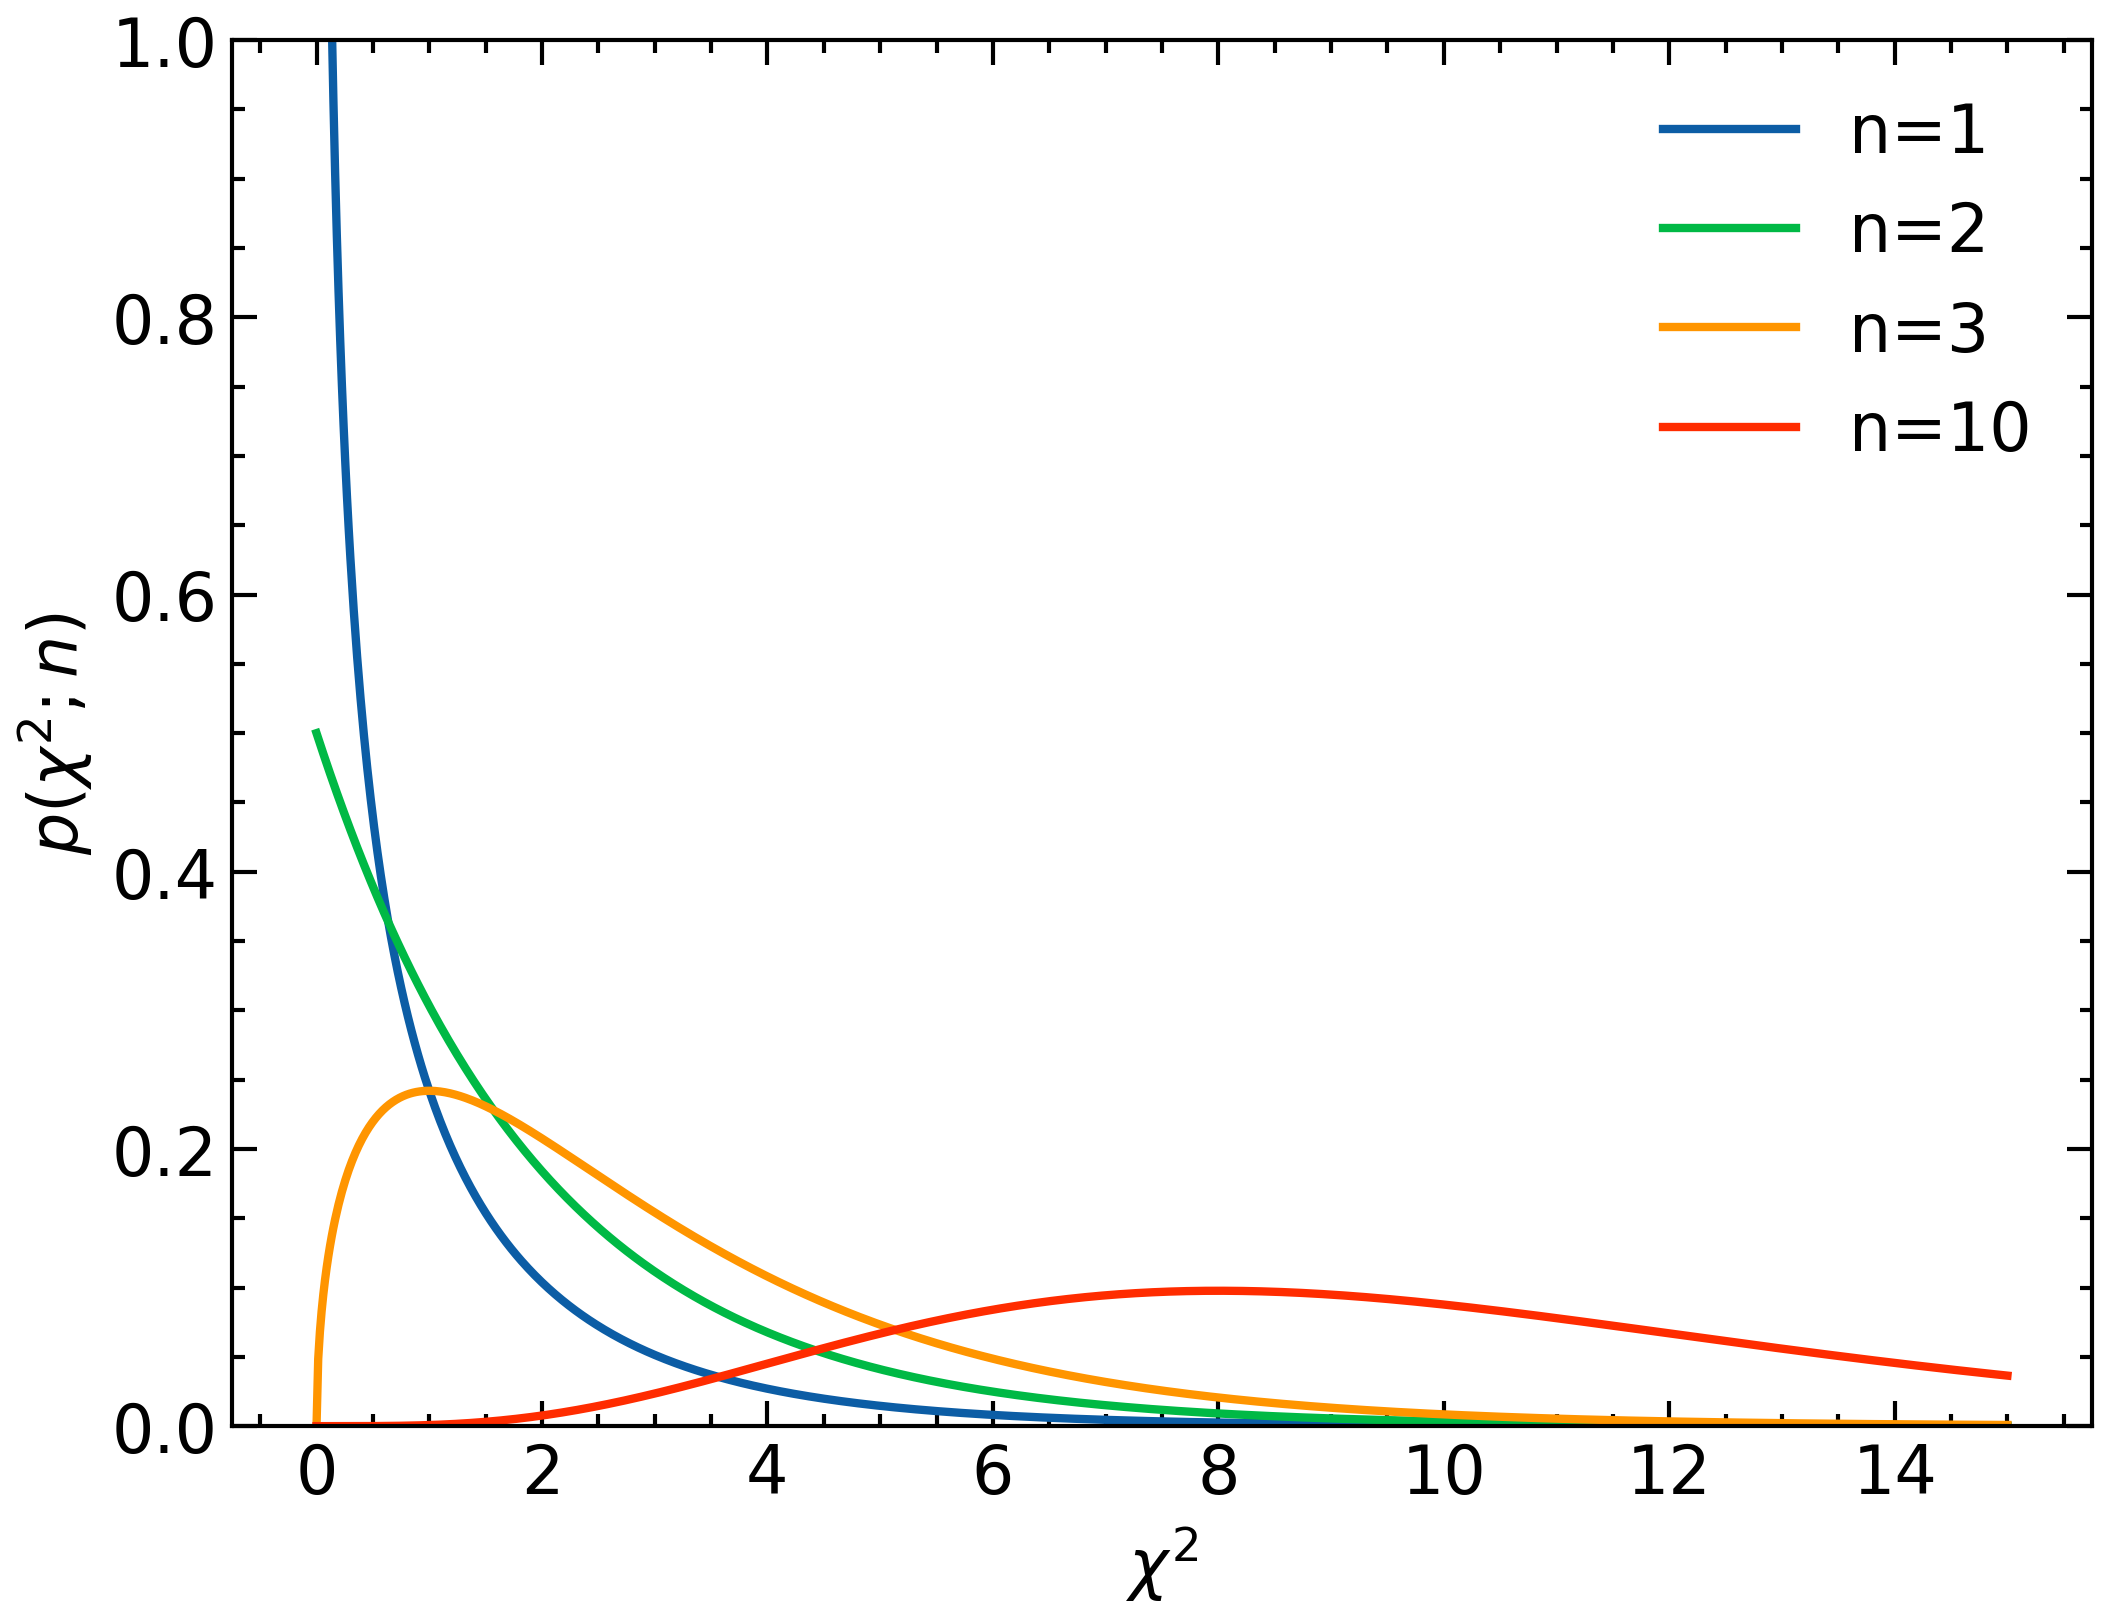
\includegraphics[width=0.7\textwidth]{hw2-p9a.png}
		      \caption{Chi-squared distribution for n=1, 2, 3, and 10 degrees of freedom.}
		      \label{fig:chi_squared_distribution}
	      \end{figure}

	\item The mode is where the pdf is at it's max. We can get these values from the plot easily but to solve it analytically, we can use the derivative of the pdf and see where it equals 0. Starting with:

	      \[ p(\chi^{2};n)=\frac{1}{2^{\frac{n}{2}}\Gamma(n/2)}(\chi^{2})^{\frac{n}{2}-1}e^{-\frac{1}{2}\chi^{2}} \]

	      \[ \dv{p(\chi^{2};n)}{\chi^{2}} = \frac{1}{2^{\frac{n}{2}}\Gamma(n/2)} \dv{\left[(\chi^{2})^{\frac{n}{2}-1}e^{-\frac{1}{2}\chi^{2}}\right]}{\chi^{2}} \]

	      Setting the derivative part to 0 using MATLAB symbolic differentiation:

	      \begin{verbatim}
			% Define symbolic variables
			syms chi_sq n positive

			% Define the expression (without normalization constant)
			expr = (chi_sq)^(n/2 - 1) * exp(-chi_sq/2);

			% Take derivative and solve for maximum
			derivative = diff(expr, chi_sq);
			[mode, params, conds] = solve(derivative == 0, chi_sq, 'ReturnConditions', true);

			% Display result
			fprintf('%s\n', latex(simplify(mode)));
			fprintf('Conditions: %s\n', latex(conds));
		  \end{verbatim}

	      \textbf{Result:}
	      \[\boxed{
			      \chi^{2}_{\text{mode}} = \begin{cases}
				      n-2 & \text{for } n \geq 2 \\
				      0   & \text{for } n < 2
			      \end{cases} }
	      \]

	\item To calculate the mean as a function of n, we can use the definition of expected value:

	      \[ \mathbb{E}(\chi^2) = \int_0^\infty \chi^2 \cdot p(\chi^2; n) d\chi^2 \]

	      where we have the given pdf

	      \[ p(\chi^{2};n)=\frac{1}{2^{\frac{n}{2}}\Gamma(n/2)}(\chi^{2})^{\frac{n}{2}-1}e^{-\frac{1}{2}\chi^{2}} \]

	      To save time I am going to use MATLAB generated code to solve this step:

	      \begin{verbatim}
			% Define symbolic variables
			syms chi_sq n positive

			% Define chi-squared PDF
			pdf = (chi_sq)^(n/2 - 1) * exp(-chi_sq/2) / (2^(n/2) * gamma(n/2));

			% Mean
			mean_chi = int(chi_sq * pdf, chi_sq, 0, inf);
			mean_chi = simplify(mean_chi);

			% Display LaTeX output
			fprintf('Mean: %s\n', latex(mean_chi));
		  \end{verbatim}

	      \textbf{Result:}

	      \[ \boxed{\mathbb{E}(\chi^2) = n} \]


	\item To calculate the variance as a function of n, we can use the definition of variance:
	      \[ V(\chi^2) = \mathbb{E}((\chi^2)^2) - (\mathbb{E}(\chi^2))^2 \]

	      where

	      \[ \mathbb{E}(\chi^2) = \int_0^\infty \chi^2 \cdot p(\chi^2; n) d\chi^2 \]
	      and
	      \[ \mathbb{E}((\chi^2)^2) = \int_0^\infty (\chi^2)^2 \cdot p(\chi^2; n) d\chi^2 \]

	      where again we have the given pdf

	      \[ p(\chi^{2};n)=\frac{1}{2^{\frac{n}{2}}\Gamma(n/2)}(\chi^{2})^{\frac{n}{2}-1}e^{-\frac{1}{2}\chi^{2}} \]


	      to save time I am going to again use MATLAB generated code to solve this step:

	      \begin{verbatim}
		  % Define symbolic variables
			syms chi_sq n positive

			% Define chi-squared PDF
			pdf = (chi_sq)^(n/2 - 1) * exp(-chi_sq/2) / (2^(n/2) * gamma(n/2));

			% Mean
			mean_chi = int(chi_sq * pdf, chi_sq, 0, inf);
			mean_chi = simplify(mean_chi);

			% Second moment
			second_moment = int(chi_sq^2 * pdf, chi_sq, 0, inf);
			second_moment = simplify(second_moment);

			% Variance
			variance = simplify(second_moment - mean_chi^2);

			% Display LaTeX output
			fprintf('Mean: %s\n', latex(mean_chi));
			fprintf('Second moment: %s\n', latex(second_moment));
			fprintf('Variance: %s\n', latex(variance));
		  \end{verbatim}

	      \textbf{Result:}

	      \[ \boxed{V(\chi^2) = 2n} \]


\end{enumerate}
\subsection*{Problem 10}
\begin{quote}
	The Exponential Distribution. The exponential probability density function is
	$$ E(x;\beta)=\frac{1}{\beta}e^{-\frac{x}{\beta}}, \quad x\ge0 $$
	\begin{enumerate}
		\item[(a)] What is the mode of this distribution?
		\item[(b)] Derive the mean.
		\item[(c)] Derive the variance.
		\item[(d)] Derive the median.
		\item[(e)] Calculate the third moment of z and use this and the previous results to derive the standard skewness $\mathbb{E}((\frac{x-\mu}{\sigma})^{3})$.
	\end{enumerate}
\end{quote}

\divider

\begin{enumerate}[label=(\alph*)]
	\item For mode we can see that the exponential distribution is a decreasing function for $x \geq 0$, so the maximum value occurs at the left endpoint of the domain, which is $x = 0$. Thus, the mode of the distribution is:

	      \[ \boxed{\text{Mode} = 0} \]
	\item To derive the mean, we use the definition of the expected value:
	      \[ \mathbb{E}(x) = \int_0^\infty x \cdot E(x;\beta) dx = \int_0^\infty x \cdot \frac{1}{\beta} e^{-\frac{x}{\beta}} dx \]

	      \begin{verbatim}
			syms x beta positive

			% Define exponential PDF
			E_x = (1/beta) * exp(-x/beta);

			% Mean
			mean_x = int(x * E_x, x, 0, inf);
			mean_x = simplify(mean_x);

			% Display
			fprintf('%s\n', latex(mean_x));
		  \end{verbatim}

	      \[ \boxed{\mathbb{E}(x) = \beta} \]

	\item To derive the variance we use the definition of the variance:
	      \[ V(x) = \mathbb{E}(x^2) - (\mathbb{E}(x))^2 \]
	      where
	      \[ \mathbb{E}(x^2) = \int_0^\infty x^2 \cdot E(x;\beta) dx = \int_0^\infty x^2 \cdot \frac{1}{\beta} e^{-\frac{x}{\beta}} dx \]
	      and we already have $\mathbb{E}(x) = \beta$ from part (b).



	      \begin{verbatim}
			syms x beta positive

			% Define exponential PDF
			E_x = (1/beta) * exp(-x/beta);

			% Second moment
			E_x2 = int(x^2 * E_x, x, 0, inf);
			E_x2 = simplify(E_x2);

			% Variance (using mean = beta from part b)
			variance = simplify(E_x2 - beta^2);

			% Display
			fprintf('Second moment: %s\n', latex(E_x2));
			fprintf('Variance: %s\n', latex(variance));
		  \end{verbatim}

	      \[ \boxed{V(x) = \beta^2} \]

	\item To derive the median, we need to find the value $m$ such that:
	      \[ \int_0^m E(x;\beta) dx = 0.5 \]

	      \begin{verbatim}		
			syms x beta m positive

			% Define exponential PDF
			E_x = (1/beta) * exp(-x/beta);

			% Compute CDF from 0 to m
			CDF = int(E_x, x, 0, m);
			CDF = simplify(CDF);

			% Solve CDF = 0.5 for median
			median_val = solve(CDF == 0.5, m);
			median_val = simplify(median_val);

			% Display
			fprintf('CDF: %s\n', latex(CDF));
			fprintf('Median: %s\n', latex(median_val));
		  \end{verbatim}

	      \[ \boxed{\text{Median} = \beta \ln(2)} \]


	\item To calculate the third moment of x, we use the definition of the expected value:
	      \[ \mathbb{E}(x^3) = \int_0^\infty x^3 \cdot E(x;\beta) dx = \int_0^\infty x^3 \cdot \frac{1}{\beta} e^{-\frac{x}{\beta}} dx \]
	      Then, to derive the standard skewness, we use the formula:
	      \[ \mathbb{E}((x-\mu)^3) = \int_0^\infty (x-\mu)^3 \cdot E(x;\beta) dx = \int_0^\infty (x-\mu)^3 \cdot \frac{1}{\beta} e^{-\frac{x}{\beta}} dx \]


	      \begin{verbatim}
			syms x beta positive

			% Define exponential PDF
			E_x = (1/beta) * exp(-x/beta);

			% Third raw moment
			E_x3 = int(x^3 * E_x, x, 0, inf);
			E_x3 = simplify(E_x3);

			% Third central moment (using mu = beta from part b)
			mu = beta;
			third_central = int((x - mu)^3 * E_x, x, 0, inf);
			third_central = simplify(third_central);

			% Standard skewness (using sigma = beta from part c)
			sigma = beta;
			skewness = simplify(third_central / sigma^3);

			% Display
			fprintf('Third moment: %s\n', latex(E_x3));
			fprintf('Third central moment: %s\n', latex(third_central));
			fprintf('Skewness: %s\n', latex(skewness));
		  \end{verbatim}

	      \[ \boxed{\text{Skewness} = 2} \]

\end{enumerate}

\end{document}
